\documentclass{PresentationHEIGVD}

\institute{} 
\title{Vaccin Peptidique contre \textit{H. Pylori}} 
\author{Nicolas Kobel, Raphaël Racine} 
\date{\today}

\setbeamertemplate{caption}{\raggedright\insertcaption\par\scriptsize}

\begin{document}

\makeheigvdtitle{, \href{mailto:nicolas.kobel@heig-vd.ch}{\color{blue}{\texttt{nicolas.kobel@heig-vd.ch}}}, \href{mailto:nicolas.kobel@heig-vd.ch}{\color{blue}{\texttt{raphael.racine@heig-vd.ch}}}}

\begin{frame}{Table des Matières}
\tableofcontents
\end{frame}

\section{Rappel}
\subsection{H. Pylori}
%\tableofcontents
\begin{frame}{Rappel}{\textit{H. Pylori}}
\begin{columns}[c]
	\begin{column}[c]{5cm}
		\begin{itemize}[<+->]
			\item Muqueuses Estomac
			\item Urease
			\item Ulcers, Cancers
		\end{itemize}
	\end{column}
	\begin{column}[c]{5cm}
	\begin{figure}
		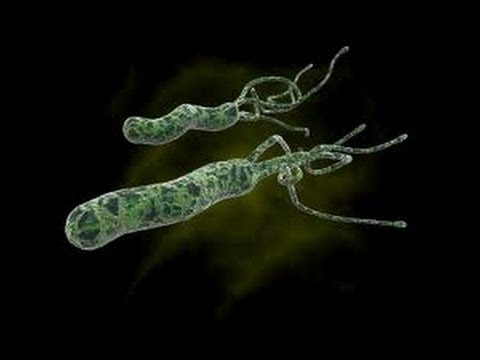
\includegraphics[width=\textwidth]{img/hpylori.jpg}
		\caption{\href{https://i.ytimg.com/vi/DYzYLTRASRM/hqdefault.jpg}{source}}
	\end{figure}
	
	\end{column}
\end{columns}
\end{frame}

\subsection{Vaccins}
\begin{frame}{Rappel}{Vaccins}
\begin{columns}[c]
	\begin{column}[c]{5cm}
		\begin{itemize}[<+->]
			\item Entrainement système immunitaire
			\item Identification de parasites
			\item Microbes affaiblis ou morts
		\end{itemize}
	\end{column}
	\begin{column}[c]{5cm}
		\begin{figure}
		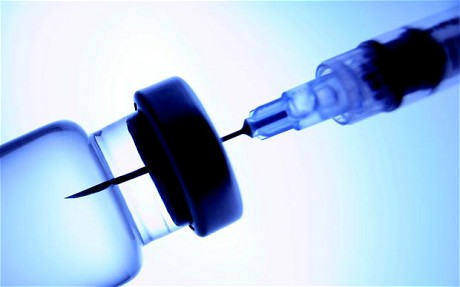
\includegraphics[width=\textwidth]{img/vaccine}
		\caption{\href{http://vaccineresistancemovement.org/wp-content/uploads/2010/05/Universal-Flu-Vaccine1.jpg}{source}}
	\end{figure}
	\end{column}
\end{columns}

\end{frame}

\subsection{Vaccins Peptidiques}
\begin{frame}{Rappel}{Vaccins Peptidiques}
\begin{columns}[c]
	\begin{column}[c]{5cm}
		\begin{itemize}[<+->]
			\item Identificateurs de la Bactérie
			\item Synthetisable
		\end{itemize}
	\end{column}
	\begin{column}[c]{5cm}	
		\begin{figure}
		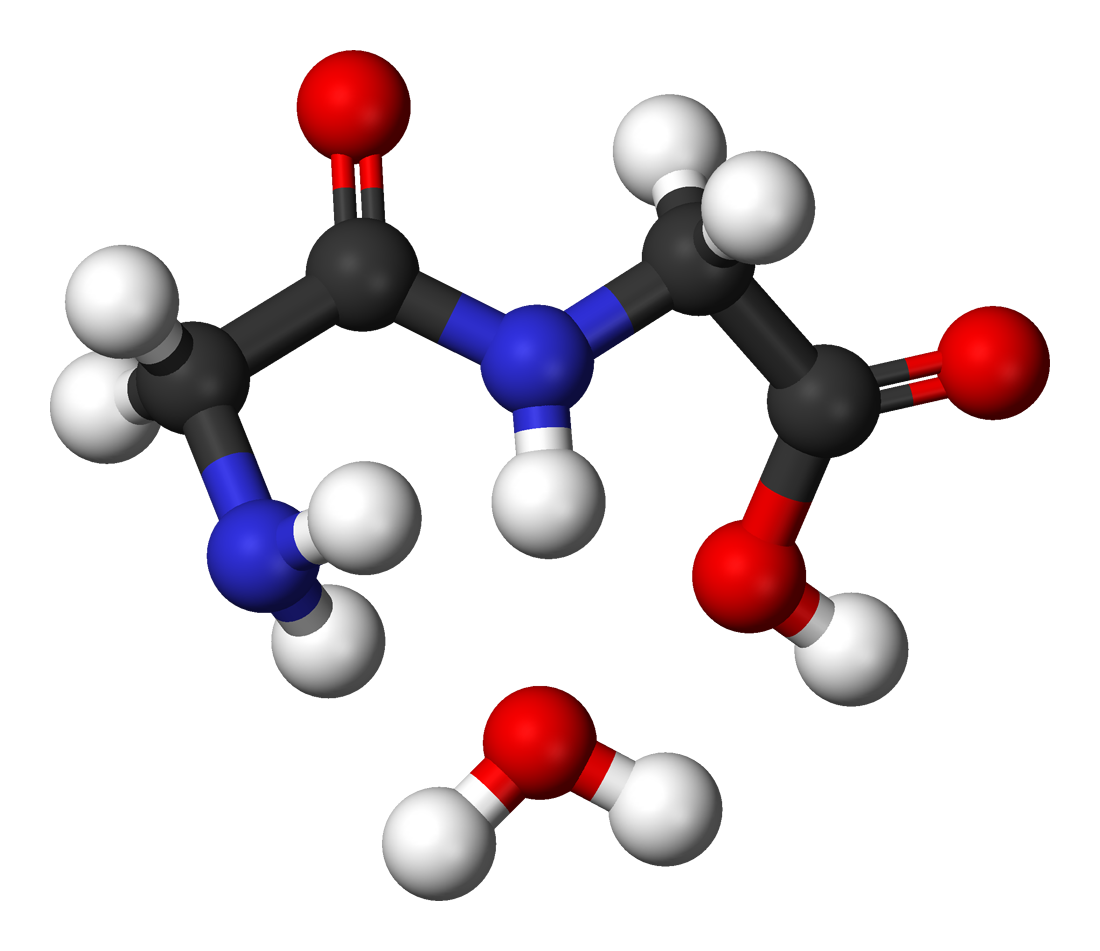
\includegraphics[width=\textwidth]{img/peptide}
		\caption{\href{https://upload.wikimedia.org/wikipedia/commons/9/94/Glycine-condensation-2-3D-balls.png}{source}}
	\end{figure}
	\end{column}
\end{columns}
\end{frame}

\subsection{Uréase}
\begin{frame}{Rappel}{Uréase}
\begin{columns}[c]
	\begin{column}[c]{5cm}
		\begin{itemize}[<+->]
			\item Utilisée pour la détéction bactérielle
			\item Deux sous unités : $\alpha$ et $\beta$
			\item $\beta$ identifieur
		\end{itemize}
	\end{column}
	\begin{column}[c]{5cm}	
		\begin{figure}
		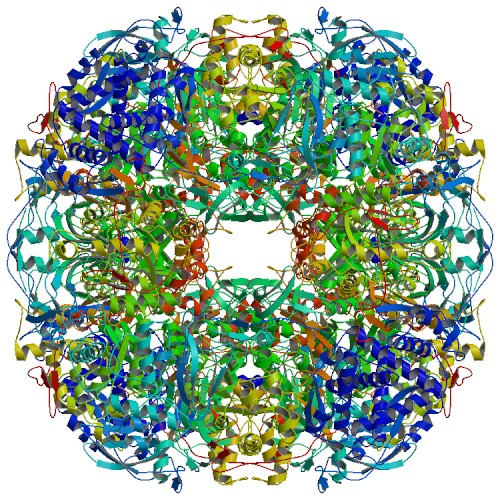
\includegraphics[width=\textwidth]{img/urease.jpg}
		\caption{\href{http://www.rcsb.org/pdb/images/1E9Z_bio_r_500.jpg}{source}}
	\end{figure}
	\end{column}
\end{columns}
\end{frame}

\subsection{Etat de l'art}
\begin{frame}{Rappel}{Etat de l'art}
\begin{columns}[c]
	\begin{column}[c]{5cm}
		\begin{itemize}[<+->]
			\item Vaccins testés en Chine
			\item Vaccin polypétpique Munich / Imevax
		\end{itemize}
	\end{column}
	\begin{column}[c]{5cm}
		\begin{figure}
		
\includegraphics[width=\textwidth]{img/imevax.png}
		\caption{\href{http://www.imevax.com/wp-content/uploads/2013/01/Imevax_Logo_V31.png}{source}}
	\end{figure}
	\end{column}
\end{columns}
\end{frame}

\section{Conception de la Solution}
\begin{frame}{Conception de la Solution}
\begin{columns}[c]
	\begin{column}[c]{5cm}
		\begin{itemize}[<+->]
			\item Prédiction d'épitopes
			\item Vérification des épitopes
			\item Liste des péptides candidats
		\end{itemize}
	\end{column}
	\begin{column}[c]{5cm}
		
	\end{column}
\end{columns}
\end{frame}

\section{Réalisation}
\begin{frame}{Réalisation}{Prédiction des épitopes}
\begin{columns}[c]
	\begin{column}[c]{5cm}
		\begin{itemize}[<+->]
			\item Deux Outils
			\item SVNTrip avec Score
			\item IEDB critère de taille
		\end{itemize}
	\end{column}
	\begin{column}[c]{5cm}
		\begin{figure}
		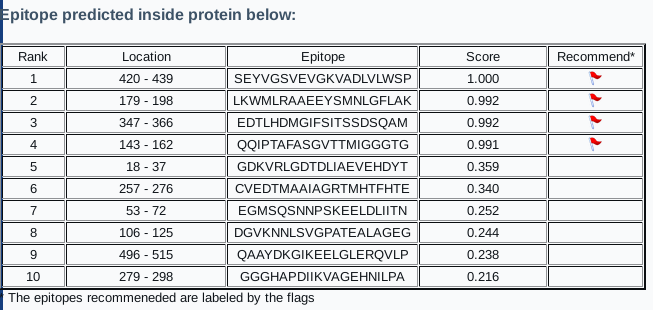
\includegraphics[width=\textwidth]{img/pred.png}
		\caption{Epitopes prédits}
		\end{figure}
	\end{column}
\end{columns}

\end{frame}

\begin{frame}{Réalisation}{Alignement}
\begin{columns}[c]
	\begin{column}[c]{5cm}
		\begin{itemize}[<+->]
			\item Recherche des Souches
			\item Alignement des Epitopes
			\item Alignement des Souches
		\end{itemize}
	\end{column}
	\begin{column}[c]{5cm}
		\begin{figure}
		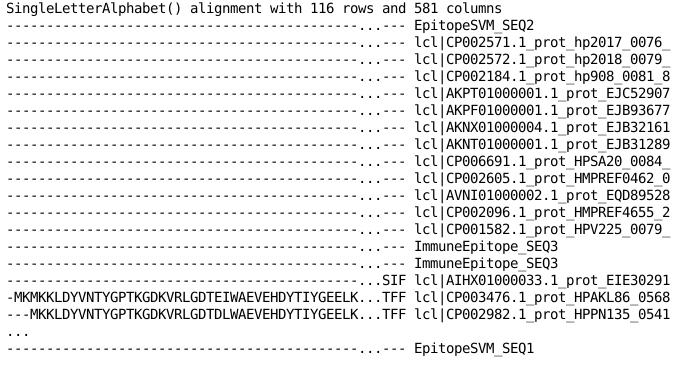
\includegraphics[width=\textwidth]{img/align.png}
		\caption{Résultats de l'alignement}
		\end{figure}
	\end{column}
\end{columns}

\end{frame}


\begin{frame}{Réalisation}{Calcul d'un score}
\begin{columns}[c]
	\begin{column}[c]{5cm}
		\begin{itemize}[<+->]
			\item Charactère par charactère
			\item Accord +1
			\item Désaccor 0
			\item Normalisation
		\end{itemize}
	\end{column}
	\begin{column}[c]{5cm}
		
	\end{column}
\end{columns}

\end{frame}

\section{Résultats}
\begin{frame}{Résultats}
\begin{columns}[c]
	\begin{column}[c]{5cm}
		\begin{itemize}[<+->]
			\item Détermination de Seuil
			\item 2 épitopes candidats
			\item Recherche d'homologues
		\end{itemize}
	\end{column}
	\begin{column}[c]{5cm}
		\begin{figure}
		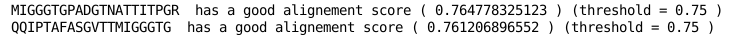
\includegraphics[width=\textwidth]{img/results.png}
		\caption{Résultats finaux}
		\end{figure}
	\end{column}
\end{columns}

\end{frame}

\section{Questions}
\begin{frame}
\frametitle{Questions}
		\begin{figure}
		
\includegraphics[height=0.6\textheight]{img/questions}
		%\caption{\href{http://www.unngls.org/images/areas-of-work/WHO.jpg}{source}}
	\end{figure}
\end{frame}

\section*{sources}


\begin{frame}[allowframebreaks]
  \frametitle<presentation>{Sources}    
  \begin{thebibliography}{10}  
    \beamertemplateonlinebibitems
  \bibitem{wiki}
    \newblock {\em Wikipedia vaccins}
    \newblock \url{https://fr.wikipedia.org/wiki/Vaccination}
    
      \beamertemplateonlinebibitems
  \bibitem{wiki2}
    \newblock {\em Wikipedia Adjuvant}
    \newblock \url{https://fr.wikipedia.org/wiki/Adjuvant}
    
          \beamertemplateonlinebibitems
  \bibitem{wiki3}
    \newblock {\em Wikipedia Epitopes}
    \newblock \url{https://fr.wikipedia.org/wiki/\%C3\%89pitope }
    
          \beamertemplateonlinebibitems
  \bibitem{wiki3}
  E-santé.fr
    \newblock {\em Article H. Pylori}
    \newblock \url{http://www.e-sante.fr/helicobacter-pylori-bacterie-tous-dangers/actualite/1534 } 
   
 \beamertemplateonlinebibitems
  \bibitem{wiki3}
  National Cancer Institute
    \newblock {\em H. Pylori and Cancer}
    \newblock \url{http://www.cancer.gov/about-cancer/causes-prevention/risk/infectious-agents/h-pylori-fact-sheet}   
    
 \beamertemplateonlinebibitems
  \bibitem{wiki3}
  MedicineNet.com
    \newblock {\em H. Pylori}
    \newblock \url{http://www.medicinenet.com/helicobacter_pylori/article.htm}      

 \beamertemplateonlinebibitems
  \bibitem{wiki3}
  Nation Institute of Health
    \newblock {\em Test for H. Pylori}
    \newblock \url{https://www.nlm.nih.gov/medlineplus/ency/article/007501.htm}   
    
   \beamertemplateonlinebibitems
  \bibitem{wiki3}
  Medscape.com
    \newblock {\em Helicobacter Pylori Infection Treatment \& Management}
    \newblock \url{http://emedicine.medscape.com/article/176938-treatment}       
        
   \beamertemplatearticlebibitems
  \bibitem{wiki3}
  Center for Disease Control and Prevention
    \newblock {\em Helicobacter Pylori Fact Sheet for Health Care Providers}
    \newblock \url{http://www.cdc.gov/ulcer/files/hpfacts.PDF}
    
       \beamertemplatearticlebibitems
  \bibitem{wiki3}
  Ming Zeng {\em et al.}
    \newblock {\em Efficacy, safety, and immunogenicity of an oral recombinant Helicobacter pylori vaccine in children in China: a randomised, double-blind, placebo-controlled, phase 3 trial}
    \newblock Lancet 2015; 386: 1457–64
    \newblock \url{http://www.thelancet.com/journals/lancet/article/PIIS0140-6736\%2815\%2960310-5/abstract}   
    
       \beamertemplateonlinebibitems
  \bibitem{wiki3}
  Technologist.eu
    \newblock {\em Towards the first Helicobacter pylori vaccine?}
    \newblock \url{http://www.technologist.eu/towards-the-first-helicobacter-pylori-vaccine/}     
    
  \beamertemplatearticlebibitems
  \bibitem{Autor1990}
    Xingdong Yang and Xinglong Yu
    \newblock {\em An introduction to epitope prediction methods
and software}.
    \newblock Rev. Med. Virol. 2009; 19: 77–96.
    \newblock \url{http://onlinelibrary.wiley.com/doi/10.1002/rmv.602/abstract}

  \end{thebibliography}
\end{frame}

\end{document}